\section{Tulokset}

Esitetyt tulokset on johdettu ohjelmissa annetuilla oletusarvoilla. Yhtälön \ref{eq:xyz_graph} muuttujat on rajoitettu välille [-20, 20] ja yhtälön
\ref{eq:sum} välille [0,20].

Kuvassa \ref{fig:graphs} on geneettisen algoritmin kulkua esittävät kuvaajat yhtälöiden \ref{eq:xyz_graph} (vasemmalla) ja \ref{eq:sum} (oikealla)
maksimointiongelmissa. Kuvaajista huomataan, että yhtälön \ref{eq:sum} (muuttujien arvot rajattu välille) maksimointiongelmassa keskimääräisen
arvo lähenee parasta mahdollista arvoa, mikä on selitettävissä yhtälön yksinkertaisuudella (kunkin muuttujan kasvattaminen
johtaa ongelman kelvollisuusarvon kasvamiseen). Kuvaajista havaitaan populaation keskimääräisen kelvollisuusarvon hitaampi kasvu RankedTournamentSelection:issa (kuvaajat 1 ja 4)
kuin muissa valintamenetelmistä, ts. kyseisessä valintamenetelmässä on populaation huonommilla jäsenillä suurempi todennäköisyys tulla valituksi, mikä
vähentää jämähtämistä lokaaleihin ääriarvopisteisiin. RouletteSelection valintamenetelmää on käytetty kuvaajissa 2 ja 5 ja RankSelection valintamenetelmää
kuvissa 3 ja 6.

\begin{figure}[H]
	\caption{Geneettisen algoritmin kulkua esittävät kuvaajat eri valintamenetelmillä}
	\centering
	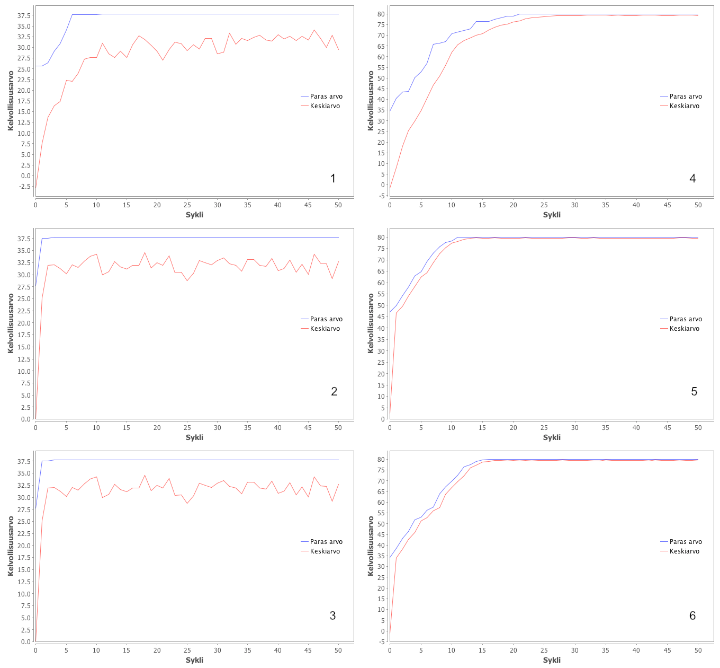
\includegraphics[width=\textwidth]{graphs}
	\label{fig:graphs}
\end{figure}

Havaittiin että yhtälön \ref{eq:xyz_graph} maksimointiongelmassa jämähdettiin joillain suorituskerroilla erääseen lokaaliin
maksimiin käytettävästä valintamenetelmästä riippumatta. Tämän huomattiin vähänevän, jos populaation kokoa kasvatettiin.
Kuitenkin parempana ratkaisuna voisi olla valintaprosessin luominen, jossa
valituksi tulemisen todennäköisyydeksi kelvollisuusarvon rinnalla otettaisiin eroavaisuus jo valituista populaation
jäsenistä. Kuvassa \ref{fig:xyz_graph_annotated} on esitetty alueet, joihin GA päätyy. Alue a on arvojoukon todellinen maksimiarvo.
Kuvaajasta huomataan, että jämähdettäessä alueelle b ei voida päätyä parempaan ratkaisuun alkioiden risteytyksellä ja mutaatiolla
se on äärimmäisen epätodennäköistä.

\begin{figure}[H]
	\caption{Saavutettu maksimikohta yhtälön \ref{eq:xyz_graph} maksimoinnissa}
	\centering
	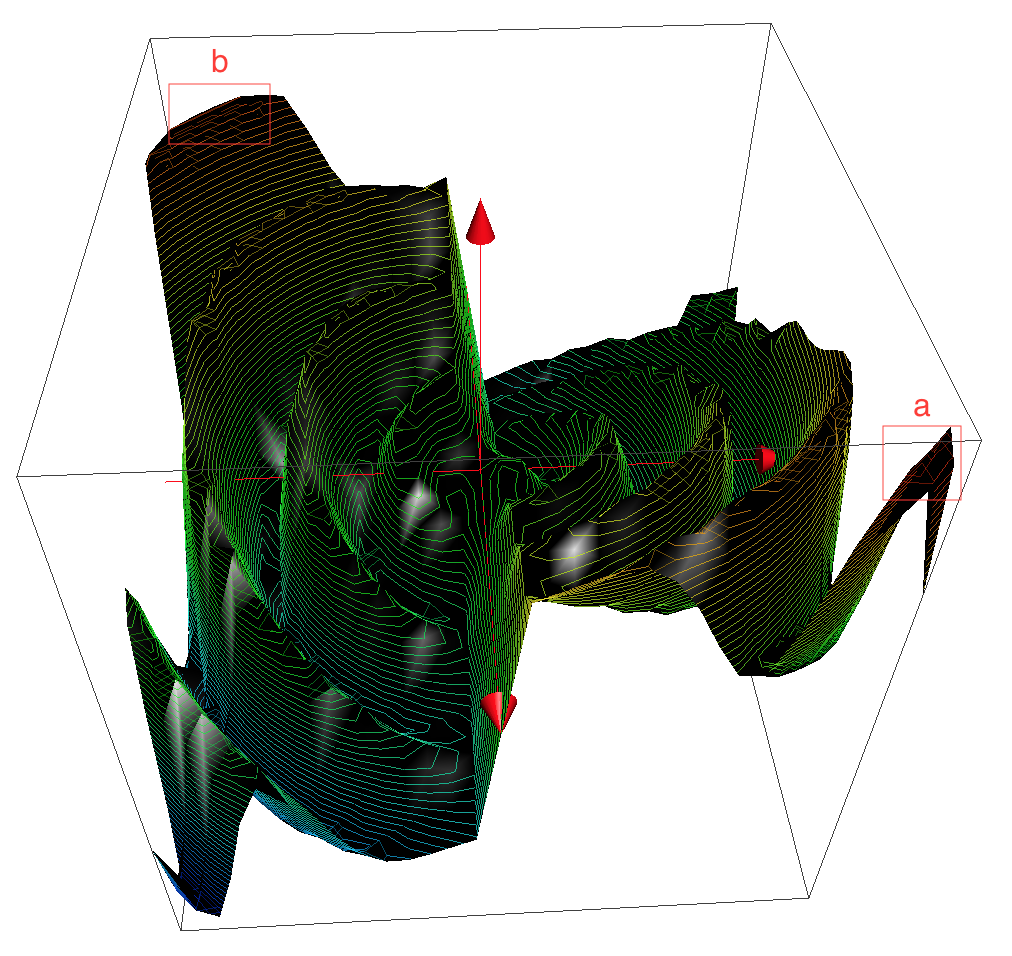
\includegraphics[width=12cm]{xyz_graph_annotated}
	\label{fig:xyz_graph_annotated}
\end{figure}
